\documentclass[11pt,a4paper]{article}
\usepackage{fontspec}
\setmainfont{Latin Modern Roman}
\setsansfont{Latin Modern Sans}
\setmonofont{Latin Modern Mono}
\usepackage[margin=2.5cm]{geometry}
\usepackage{graphicx,booktabs,tabularx,longtable,array,amsmath,amssymb}
\usepackage{caption,float,placeins,enumitem,xstring}
\usepackage[numbers,sort&compress]{natbib}
\usepackage[hidelinks,unicode]{hyperref}
\usepackage{doi}
% Điền thông tin nhóm tại đây; file này dùng chung cho report và slide.
\newcommand{\ProjectName}{ResearchLens}
\newcommand{\ProjectSubtitle}{Intelligent Research Paper Search and Discovery System}
\newcommand{\CourseName}{IT4868E -- Web Mining}
\newcommand{\Semester}{2026.1}
\newcommand{\TeamName}{Nhóm ResearchLens}
\newcommand{\TeamMembers}{Thông tin thành viên và MSSV: bổ sung trước khi nộp}
\newcommand{\Instructor}{TS. Nguyễn Kiêm Hiếu}
\newcommand{\ReportDate}{14 tháng 10 năm 2026}

\newcommand{\CatalogCount}{129.596}
\newcommand{\CatalogLatencyMedian}{44.2}
\newcommand{\CatalogLatencyTail}{153.2}
\newcommand{\CatalogBuildSeconds}{7.7}
\newcommand{\CatalogIndexMiB}{525.9}
\newcommand{\CatalogAbstractPercent}{73.1}

\newcommand{\CatalogCountEn}{\StrSubstitute{\CatalogCount}{.}{,}}
\captionsetup{font=small}
\setlist{itemsep=2pt}
\graphicspath{{../artifacts/figures/report/}{../artifacts/screenshots/}}
\hypersetup{pdftitle={ResearchLens: Recommending What to Read Next from a Library of Saved Papers},pdfauthor={Group 5: Tran Quang Hung, Vu Thuong Tin, Chu Anh Duc, Dinh Quoc Bao}}
\makeatletter
\newcommand{\tableinput}[1]{\@@input#1 }
\makeatother
\newcommand{\fig}[4]{\begin{figure}[htbp]\centering\includegraphics[width=#2\linewidth]{#1}\caption{#3}\label{#4}\end{figure}}

\begin{document}
\begin{titlepage}
\centering

\includegraphics[width=12cm]{images/hust-logo.png}\par
\vspace{0.8cm}

\includegraphics[width=5cm]{images/soict-logo.png}\par
\vspace{1.4cm}
{\large Course project report\par}
\vspace{0.3cm}
{\large IT4868E Web Mining, semester \Semester\par}
\vspace{1.6cm}
{\LARGE\bfseries ResearchLens\par}
\vspace{0.5cm}
{\Large Recommending What to Read Next\\from a Library of Saved Papers\par}
\vspace{2.5cm}
\begin{tabular}{@{}rl@{}}
Instructor: & Dr. Nguyễn Kiêm Hiếu\\
Group: & 5\\
Members: & Tran Quang Hung, 20235502\\
 & Vu Thuong Tin, 20230091\\
 & Chu Anh Duc, 20230081\\
 & Dinh Quoc Bao, 20235478\\
\end{tabular}
\vfill
{\large Hanoi, November 2026\par}
\end{titlepage}

\begin{abstract}
A researcher who has saved a few papers on a topic needs to decide what to read next. ResearchLens takes that library and ranks every other paper in a corpus of 3,595 papers with 13,481 internal citation edges and 1,320 scored peer reviews. Each recommendation comes with evidence the reader can check: the papers that cite it together with a saved paper, its citation links to the library, and reviews of it with the original sentences.

We have no logs of real readers, so we evaluate on surrogate tasks. In the main experiment (E2) we cut the corpus at the end of 2020, hide one third of the references of each of 219 later papers, and ask each method to recover them from the rest. Cocitation is the best single signal, with nDCG@10 of 0.173. Reciprocal rank fusion of cocitation with a content and PageRank hybrid reaches 0.207, against 0.143 for the hybrid alone (+0.064 [0.042, 0.087]). On a random edge holdout (E3) fusion again beats the hybrid but loses to cocitation alone, so we only claim that fusion is better than the hybrid. On a task closer to real reading (E2b), predicting the papers 250 authors cite for the first time after 2020, every method scores lower and fusion still leads among the methods of the app.

A gradient boosting model trained on 2,081 tasks generated from cutoffs between 2010 and 2018 reaches 0.224, 0.132 and 0.297 on the three tasks and beats fusion on all three, with intervals above zero on two. When the reader also describes a topic in one sentence, a version of the model that adds BM25 retrieval reaches 0.237, 0.182 and 0.304 and beats fusion with intervals above zero on all three. In terms of Hit@10, the share of tasks with at least one right paper in the first ten, that model reaches 64\%, 58\% and 78\%, against 58\%, 42\% and 71\% for fusion. The app uses this decision model by default; one request takes 85\,ms at the median.

We also asked language models to rank. On the same candidates, a 1.5B small model and a text only LLM rank worse than the decision model. An LLM given citation evidence for each of 100 candidates (graph RAG) reaches 0.242, 0.135 and 0.310, slightly above the decision model on the same candidates, with intervals that include zero, at about 200 seconds per request. In the app a small model (Qwen2.5 0.5B on CPU) only writes a one sentence summary of the recommended paper from its abstract; 17 of 20 sentences we checked by hand were correct. On 115 PeerRead test reviews, TF-IDF with logistic regression reaches macro F1 of 0.469 for labels derived from review scores. On 300 SciFact queries, BM25 reaches nDCG@10 of 0.651 against 0.621 for TF-IDF.

\medskip\noindent\textbf{Keywords:} paper recommendation, citation network, cocitation, reciprocal rank fusion, learning to rank, retrieval augmented generation, opinion mining.
\end{abstract}

\clearpage
\tableofcontents
\clearpage
\listoffigures
\listoftables
\clearpage

\section{Introduction}\label{sec:intro}
Someone starting a project usually has a handful of relevant papers and wants to know which one to read next. ResearchLens is built around that moment. The reader saves papers into a library $S$, and the system ranks every other paper in the corpus. A saved paper is never recommended again. Every recommendation shows why it was made: the papers that cite it together with a saved paper, its citation links to the library, the words it shares with the library, and the reviews of it with the original sentences. Search, the citation graph, projects and the PDF reader are the steps around this task. Readers find and save papers, get recommendations, and then open a paper to read its abstract, its reviews and its citation neighborhood before they decide.

We do not have logs of what real readers did, so we use surrogate tasks. We hide part of the reference list of a paper, give the rest to the system as the library, and count how many hidden references it recovers. Citation recommendation research has used this protocol for a long time \citep{mcnee2002,strohman2007}. It has a weakness that matters for this report. The answers are references, and cocitation is built from references, so the protocol favors citation signals. The answers are also papers the authors already knew when they wrote, not papers they had not yet read. We therefore add a second task closer to real reading: from the papers an author wrote up to 2020, predict the papers that author cites for the first time after 2020.

The report answers two questions.
\begin{enumerate}
\item \textbf{RQ1.} Which signal recovers the hidden papers best: popularity, TF-IDF content, Personalized PageRank or cocitation?
\item \textbf{RQ2.} Does a combination of signals beat the best single signal? We compare a linear hybrid of content and PageRank, rank fusion of cocitation with that hybrid, learned rerankers, and the effect of MMR on relevance and diversity.
\end{enumerate}
Two other parts of the system are checked because they are shown next to recommendations. The review classifier is tested on PeerRead (E4), and lexical retrieval is tested on SciFact (E1), because search is how readers save their first papers. Experiments for the passage search inside the reader concern retrieval, use few queries, and are reported in Appendix~\ref{app:reader}.

The course syllabus places the project in link analysis, opinion mining or recommender systems, and excludes projects that are only about information retrieval. Retrieval is therefore the access layer of the system, and the experimental work is about link mining, recommendation and reviews. The report follows two input documents: the visual specification of the project, which describes the workflow and a scope of 2,000 to 5,000 AI and ML papers, and the course syllabus.

Section~\ref{sec:related} reviews related work. Sections~\ref{sec:data} and~\ref{sec:system} describe the data and the system, Section~\ref{sec:methods} the mining methods, Section~\ref{sec:setup} the experiments and Section~\ref{sec:results} the results. Section~\ref{sec:discussion} discusses what the results support and what they do not.

\section{Related work}\label{sec:related}
\paragraph{Citation based recommendation.} \citet{small1973} proposed cocitation, the number of papers that cite two documents together, as a measure of how related they are. \citet{mcnee2002} recommended citations for a paper from its existing references and compared collaborative filtering with graph methods on hidden references, the protocol we use in E2 and E3. \citet{strohman2007} retrieved candidates with text and citation features and reranked them with a learned linear model; our learned rerankers and the topic variant of the decision model follow the same two step design. \citet{beel2016} surveyed research paper recommender systems and found that offline results often fail to predict what users prefer, which is the main limit of every number in this report.

\paragraph{Link analysis.} PageRank \citep{page1999} scores a node by the stationary distribution of a random walk with restarts; with restarts on the saved papers it becomes Personalized PageRank. HITS \citep{kleinberg1999} separates hubs from authorities. Louvain \citep{blondel2008} finds communities by greedy modularity optimization. We use NetworkX \citep{networkx} for PageRank and Louvain.

\paragraph{Combining rankings.} Reciprocal rank fusion \citep{cormack2009} adds the inverse ranks of several systems and needs no score calibration. MMR \citep{carbonell1998} trades relevance against redundancy when it picks each next item. Gradient boosting \citep{friedman2001} is the learner behind our decision model.

\paragraph{Text representations and retrieval.} We use TF-IDF and BM25 as described by \citet{manning2008} and \citet{robertson2009}. SPECTER \citep{cohan2020} learns document embeddings from citations; we test it as a replacement for TF-IDF content vectors. SciFact \citep{wadden2020} in the BEIR collection \citep{thakur2021} gives us relevance judgments for scientific claims.

\paragraph{Language models as rankers.} \citet{sun2023rankgpt} showed that an instruction tuned LLM can rerank a numbered list of passages in one call. We apply that listwise prompt to paper recommendation, with and without citation evidence retrieved from the graph for each candidate.

\paragraph{Reviews.} PeerRead \citep{kang2018,peerreadrepo} released peer reviews with scores for several venues. We use its ICLR 2017 part and derive polarity labels from the review scores.

\section{Data}\label{sec:data}
\subsection{Sources and sampling}
OpenAlex \citep{openalex} provides work metadata and the list of referenced works. We ran eight queries: graph neural networks, information retrieval, recommender systems, sentiment analysis, large language models, deep learning, reinforcement learning and knowledge graphs. Each query took the first 400 results by relevance, in English, published no later than 31 December 2025. The union by OpenAlex ID gave 3,171 works.

PeerRead reviews come from a fixed version of the public repository, ICLR 2017 part. We matched PeerRead papers to OpenAlex works by lowercased titles with punctuation removed. Three titles matched; the other 424 papers were added as new records. This is an exact join on normalized titles, not semantic entity resolution, so some title variants may remain separate.

The OpenReview API refused our requests with an access check during collection, so we used the public PeerRead snapshot and kept the source path of every review. We did not generate reviews or work around the check. The specification also lists arXiv as a source. We did not build an arXiv crawler, because the OpenAlex corpus already covered the scope and the three kinds of data we needed; this is a scoping decision, and the report does not claim that every source in the specification is integrated.

\subsection{Cleaning and provenance}
We rebuilt abstracts from the OpenAlex inverted index, normalized author lists, kept DOI, URL, venue, year and topics, removed duplicate IDs and mapped references to one ID scheme. Only edges with both ends in the corpus enter the graph, and self citations of a paper to itself are dropped. A missing abstract stays empty; we never fill it with guessed text.

A review is kept when it has text, has a recommendation score that parses as a number and is not a metareview. Repeated copies of a review for the same paper were removed after normalizing case and whitespace, which reduced 2,642 reviews to 1,320. The official PeerRead splits are kept. The data is stored as JSON lines and split on line feeds only, because some Unicode characters inside review text would otherwise break a record in two.

A provenance record keeps the collection time, the queries, the PeerRead commit and checksums of the corpus and review files. Raw API responses are cached, so normalization can run again without the network. Each normalized file is written to a temporary file and then renamed; there is no transaction across files.

\begin{table}[htbp]\centering
\begin{tabular}{@{}lr@{}}\toprule
Property & Value\\\midrule
OpenAlex papers / PeerRead papers added & 3,171 / 424\\
Papers in the merged corpus & 3,595\\
Papers with an abstract & 2,725 (75.80\%)\\
Directed internal citation edges & 13,481\\
Scored reviews after deduplication & 1,320\\
Reviews in train / dev / test & 1,082 / 123 / 115\\
Isolated nodes / largest weakly connected component & 770 / 2,798\\
Louvain communities, singletons included & 787\\\bottomrule
\end{tabular}\caption{Snapshot of 14 October 2026, measured on the delivered data.}\label{tab:data}\end{table}
\fig{corpus.pdf}{1}{The corpus by first collection query and by publication year. The sample follows search relevance and does not represent research output as a whole.}{fig:corpus}

\subsection{Entities and relations}
A paper has a stable ID, title, abstract, authors, year, venue, DOI, URL, topics, citations and references. We keep two citation counts: the count that OpenAlex reports for the whole literature, and the indegree in our graph. The two are never used in place of each other. A review links to its paper through the paper ID and keeps the original score, so the derived label can be explained.

SQLite holds the papers, the saved papers and a short query history. A saved row holds a profile, a paper ID and the time of saving. The pair of profile and paper is the primary key, so saving twice does not duplicate data, and a foreign key requires the paper to exist. When the corpus changes, the API drops saved IDs that are no longer in the engine before it builds a profile.

\subsection{Biases and limits}
Taking the first 400 results of each query introduces selection bias, and the fields are not sampled in proportion to their output. Papers without an abstract are still retrieved by title and therefore have short content vectors. Many PeerRead papers have no OpenAlex citation links, which increases the number of isolated nodes. For that reason the 787 communities are not 787 research topics. Results about the network describe the observed graph only.

\section{System}\label{sec:system}
\subsection{Architecture}
\fig{architecture.pdf}{1}{Architecture. Public data is cleaned and cached, the mining core serves the workspace, and the experiment scripts write the artifacts used in this report. Solr is an optional backend.}{fig:architecture}
FastAPI serves a synchronous API for the CPU bound work and the HTML, CSS and JavaScript interface from the same origin (Figure~\ref{fig:architecture}). SQLite stores personal libraries. The sparse matrices and the graph are built in memory at startup. scikit-learn does the vectorizing and the classifiers, and NetworkX computes PageRank and Louvain. HITS uses nonnegative power iteration on the adjacency matrix, which gives stable authority and hub directions.

This design fits a few thousand papers and needs no GPU. We did not use Spark, because at this size it adds setup cost without changing any result. For a dedicated search engine, a Docker profile adds Apache Solr 9.9.0 with the Lucene inverted index and BM25 \citep{solr}. Solr was indexed and tested on the whole corpus, but the BM25 numbers in this report come from the local sparse implementation and are not Solr measurements.

\subsection{Request flow and security}
A query goes through validation, phrase and exclusion parsing, vectorizing, lexical scoring, metadata filters and ranking. The API returns the result count, the processing time and the score components. Opening a paper also returns its keywords, entity mentions, local references, local citing papers, graph metrics and linked reviews.

The library uses a random 256 bit cookie with the HttpOnly flag and SameSite set to Strict. This is an anonymous browser profile, not a login account. Writes from another origin are rejected, SQL uses parameters, the interface escapes text and opens only HTTP or HTTPS links, and the API bounds query length, seed count, page size and value ranges. The server never unpickles uploads or executes text taken from papers or reviews.

\subsection{Interface}
The interface has views for search, the conference catalog, online search, projects, paper reading, the citation network, review insights, the library and a research dashboard. Each paper shows its source, year, venue and original link; papers in the mining workspace also show their influence in the local graph. In the graph view the reader can select, zoom, pan and open an ego network. Node size encodes PageRank and color encodes the Louvain community when groups are on. All screenshots in this report come from the delivered build.
\fig{discover.png}{1}{Search view with query, filters, lexical and graph ranking, over real papers in the corpus.}{fig:discover}
\fig{../artifacts/screenshots/network.png}{1}{Citation network view. Each edge is an observed reference and points from the citing paper to the cited paper.}{fig:networkui}
\FloatBarrier

\paragraph{Projects.} A project has a title, a short brief and a set of papers chosen by the reader. The brief is reduced to at most 32 words from the indexed vocabulary, and BM25 retrieves related papers, leaving out papers already in the project and duplicate titles. The interface shows which words of the brief appear in each paper, so the reader can see why it was suggested. We have no labels for this feature, so we make no claim about its quality. A project keeps a reading list with three states (to read, reading, read). Its citation map is the subgraph induced by its papers and can be expanded to neighbors; edges are still observed citations, and adding a paper to a project never adds an edge.
\begin{figure}[htbp]\centering

\includegraphics[width=.96\textwidth]{projects.png}
\caption{A project from the browser test. The example brief can be edited; papers and edges come from the corpus. Node positions are a layout and do not encode semantic distance.}\label{fig:projects}
\end{figure}

\paragraph{Reading PDFs and notes.} The reading view shows the original PDF in the browser viewer next to the reader's notes and the citation neighborhood. Notes hold up to 30,000 characters and a page bookmark. PDFs are fetched only from the URL in the metadata and only from allowed HTTPS repository hosts. Every redirect is checked again, and the server enforces a 20 MiB limit, a timeout and the PDF signature. When no PDF is available, the view says so and shows the abstract instead of pretending to show the full text. Notes save automatically, and a local draft survives a failed save. The browser test read a real arXiv PDF, saved 22,000 Vietnamese characters (more than 64 KiB of encoded text), reloaded, and restored a draft after a simulated failure.
\begin{figure}[htbp]\centering
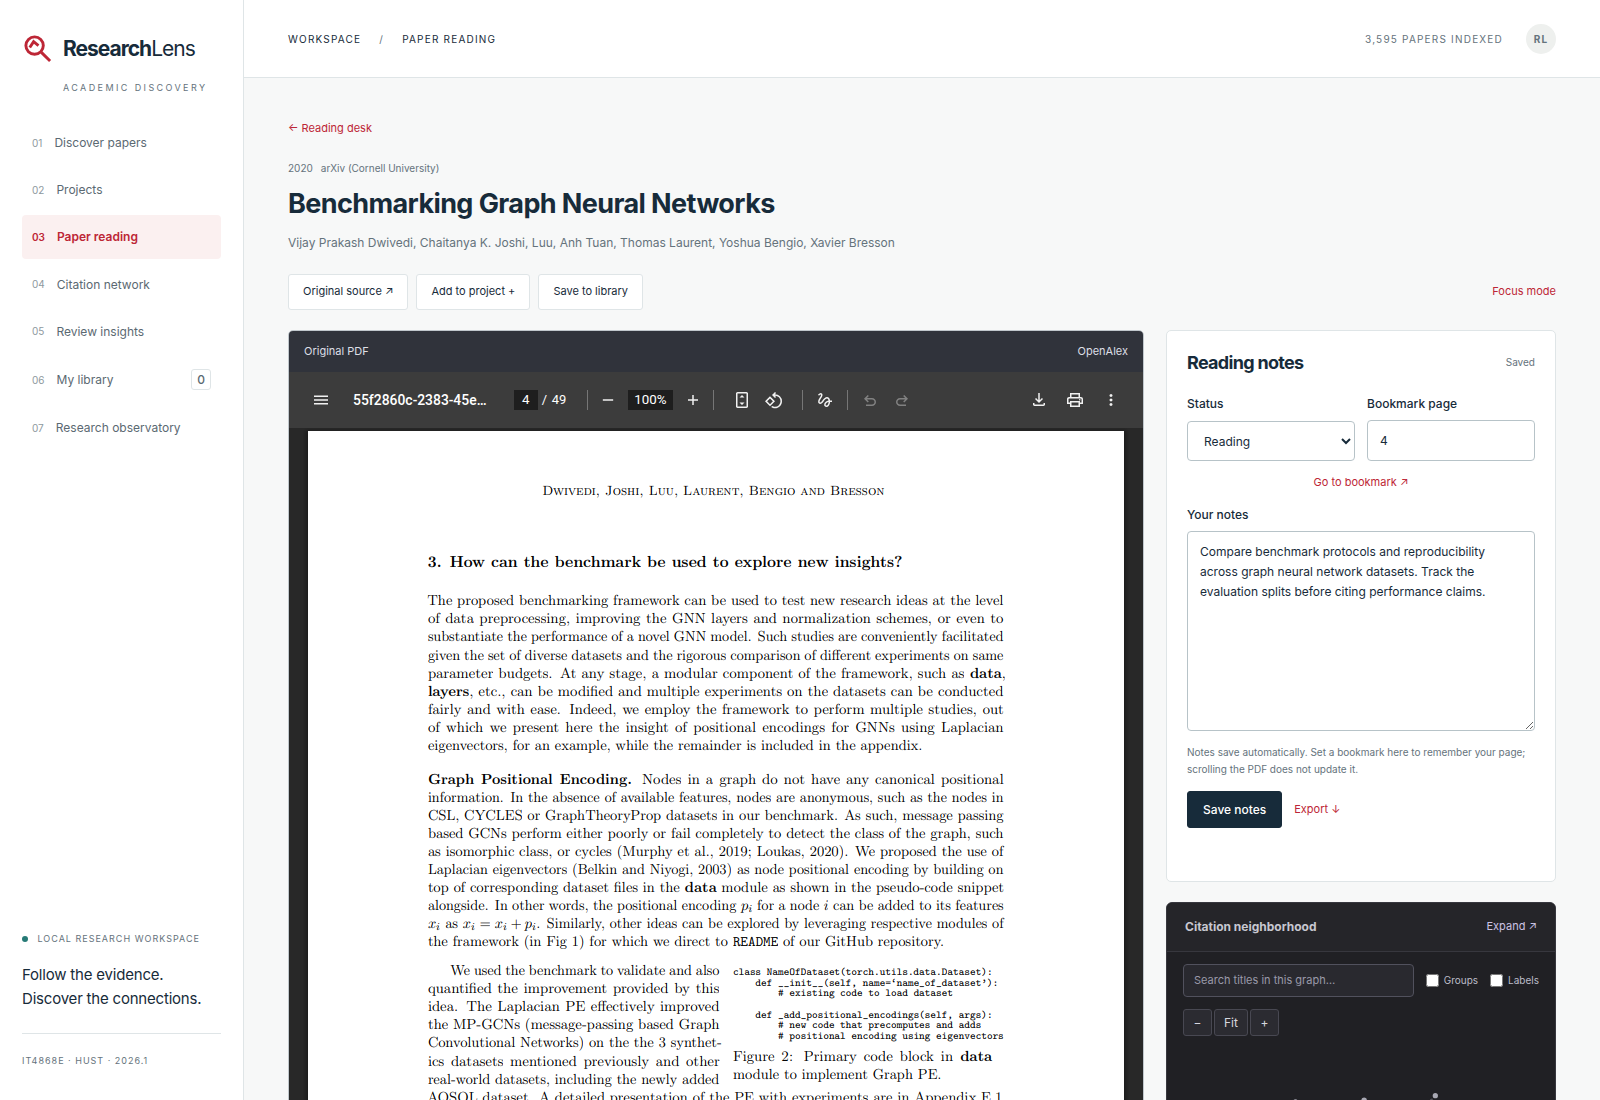
\includegraphics[width=.96\textwidth]{reading.png}
\caption{The original PDF at bookmarked page 4, next to the reader's notes. The note text is from the demo and is not used as an experimental label.}\label{fig:reading}
\end{figure}

\paragraph{Graph interaction.} The graph uses small nodes and thin edges and highlights neighbors on hover or selection. Dragging a node moves its neighbors through spring forces that settle after release. The reader can search nodes by title, pan, zoom, color by Louvain group, toggle labels and open the reader from a node. Edges keep the citing to cited direction, and a view holds at most 200 nodes. The visual design follows a public design guide and the interaction model of the Obsidian graph view; both were used as references, not as runtime libraries. Animations are turned off when the operating system asks for reduced motion.

\subsection{Kho hội nghị 2020--2026 và tìm kiếm ngoài snapshot}
Pipeline mở rộng thu thập metadata ICML, NeurIPS, ICLR, AAAI, EMNLP, NAACL, ACL và CVPR. ICML dùng volume PMLR; ICLR/NeurIPS dùng JSON của chương trình chính thức; ACL-family dùng XML ở commit cố định của ACL Anthology, gồm Findings theo đúng volume hội nghị; CVPR dùng CVF Open Access. OpenAlex bổ sung metadata qua source ID và cursor đến hết kết quả; AAAI hiện dùng nguồn này. URL từng lần fetch, trạng thái nguồn và SHA-256 của JSONL nằm trong manifest.

Collector có gzip cache theo URL, retry có giới hạn và ba worker. Khi chạy lại, dữ liệu đã tải được tái sử dụng. Bộ đọc nhận dạng khác biệt giữa program cũ/mới, loại session cha, loại workshop trong program và nối các trang CVPR theo ngày. Chuẩn hóa tiêu đề được dùng để khử trùng trong từng hội nghị/năm; giữ OpenAlex ID nếu có để nối references. Alias chính thức được lưu cùng bản ghi. Phép join này có thể bỏ sót biến thể tiêu đề hoặc hợp nhất nhầm tên giống nhau; chưa có fuzzy entity resolution.

Snapshot mở rộng chứa \CatalogCount{} bản ghi, trong đó \CatalogAbstractPercent\% có abstract. Đây là số metadata thu được từ các nguồn đã hoàn tất, không phải tổng số paper được chấp nhận đã kiểm chứng độc lập. Phạm vi có thể gồm Findings, short paper hoặc track khác được nguồn công bố. EMNLP 2026 và NAACL 2020/2023/2026 chưa có bản ghi từ các adapter tại thời điểm thu thập; ô 0 không được diễn giải thành hội nghị không tồn tại. Không tải hàng loạt PDF.
\fig{conference_coverage.pdf}{1}{Coverage sau khử trùng của snapshot mở rộng. Các số là bản ghi thu thập được; không trộn vào corpus 3.595 paper của thí nghiệm gốc.}
\FloatBarrier

Kho hội nghị dùng inverted index FTS5 trên đĩa \cite{fts5}, với trọng số BM25 cho title/abstract/authors/conference lần lượt là 8/2/2/1. Query được tách thành tối đa 32 token, nối OR, kết hợp bộ lọc hội nghị/năm và phân trang. Không đưa toàn bộ hơn một trăm nghìn paper vào NetworkX hoặc ma trận recommendation lúc startup. API truy hồi và giao diện hiển thị rõ backend này khác ranking trong mining workspace.
\begin{figure}[H]\centering

\includegraphics[width=\textwidth]{conferences.png}
\caption{Tìm kiếm thật trên kho hội nghị: query graph neural networks, ICML 2025. Abstract hoặc citation count thiếu được ghi rõ; không sinh nội dung thay thế.}
\end{figure}

Search online gửi query và lọc năm đến OpenAlex \cite{openalexsearch}, cache metadata năm phút, giới hạn 128 cache entries. API key tùy chọn nằm ở server; lỗi quota hoặc metadata sai kiểu được trả thành lỗi dịch vụ có kiểm soát. Kết quả chưa tự gia nhập graph. Nút \textit{Import \& read} lấy lại metadata từ provider theo ID, khử trùng DOI/tiêu đề và lưu bền. Với record chính thức, hệ thống thử tìm exact match để bổ sung abstract/references; nếu không có, giao diện thông báo giới hạn enrichment.

Import tạo một mining engine mới trước khi ghi/swap; lock tuần tự hóa các import trong một process. Mapping alias được áp dụng lên references cả khi import và khi khởi động lại. Nhờ vậy paper có OpenAlex ID khác với ID chính thức vẫn nối đúng cạnh citation. Corpus import dùng chung trong instance; Project, notes và thư viện vẫn riêng theo profile trình duyệt. Chưa hỗ trợ đồng bộ engine giữa nhiều worker. Apache Solr tùy chọn tiếp tục index snapshot gốc, không tự nhận paper import.
\begin{figure}[H]\centering

\includegraphics[width=\textwidth]{online_search.png}
\caption{Search online với metadata OpenAlex thật. Paper có thể import vào reader, thêm vào Project và tham gia citation graph nếu có reference khớp. Không tạo cạnh khi nguồn không cung cấp bằng chứng.}
\end{figure}

\subsection{Đo hiệu năng riêng cho kho hội nghị}
Script \texttt{scripts/evaluate\_catalog.py} dựng index mới và đo 20 query chủ đề cố định qua năm vòng, tổng cộng 100 lần đo. Mỗi query được warm một lần; các vòng xen kẽ có/không lọc hội nghị. Phạm vi gồm đếm kết quả, BM25, top-20 và giải mã JSON; không gồm HTTP, browser hoặc mạng. Trên môi trường lưu trong artifact, dựng index mất \CatalogBuildSeconds{} giây, database chiếm \CatalogIndexMiB{} MiB; latency p50 là \CatalogLatencyMedian{} ms, p95 là \CatalogLatencyTail{} ms.

Đây là phép đo mô tả trên một máy, single process, không phải load test hay kết luận về relevance. Tất cả 100 quan sát nằm trong \texttt{artifacts/catalog\_results.json}. Chưa có nhãn relevance cho kho mới nên không gán nDCG của SciFact hoặc reference recovery cũ cho 129 nghìn record này. Import thay đổi thống kê workspace đang chạy, nhưng không thay JSONL hay số đo benchmark gốc.


\section{Methods}\label{sec:methods}
\subsection{Text representation and retrieval}
The indexed text is the title twice followed by the abstract. The tokenizer lowercases, keeps alphanumeric tokens of at least two characters and removes English stopwords. The vocabulary has at most 60,000 terms, and there is no stemming in the local backend. TF-IDF vectors use sublinear term frequency and unit L2 length \citep{manning2008}:
\begin{equation}
\mathrm{tf}(t,d)=1+\log f(t,d),\qquad
\mathrm{idf}(t)=\log\frac{1+N}{1+\mathrm{df}(t)}+1.
\end{equation}
The TF-IDF score is the cosine between query and paper. BM25 uses the nonnegative IDF \citep{robertson2009}:
\begin{equation}
\mathrm{BM25}(q,d)=\sum_{t\in q}\log\left(1+\frac{N-\mathrm{df}(t)+0.5}{\mathrm{df}(t)+0.5}\right)
\frac{f(t,d)(k_1+1)}{f(t,d)+k_1(1-b+b|d|/\overline{|d|})},
\end{equation}
with $k_1=1.5$ and $b=0.75$, fixed before any benchmark. A repeated query term counts once.

Words without operators are joined with OR. A quoted phrase must appear as a phrase, a minus sign excludes a word or phrase at word boundaries, and AND requires every content token. This is a small convenience syntax, not a full Boolean language with nesting. An empty query returns PageRank order. A query with no known token returns nothing rather than an unrelated list. Search ranks by $0.85\,\widehat{s}_{\mathrm{BM25}}+0.15\,\widehat{\mathrm{PR}}$, where the hat means division by the largest value of that component. We have no relevance judgments on our own corpus, so we make no claim about this search ranking.

\subsection{PageRank, HITS and communities}
The graph $G=(V,E)$ has an edge $u\rightarrow v$ when paper $u$ cites paper $v$. With damping $\alpha=0.85$, PageRank \citep{page1999} satisfies
\begin{equation}
\pi(v)=(1-\alpha)p(v)+\alpha\sum_{u:(u,v)\in E}\frac{\pi(u)}{\deg^+(u)}.
\end{equation}
Global PageRank uses a uniform $p$; Personalized PageRank spreads the restart mass evenly over the saved papers. A high score reflects position in the observed network, not correctness or quality. HITS \citep{kleinberg1999} iterates $a\leftarrow A^\top h$ and $h\leftarrow Aa$ with normalization after each step. Louvain \citep{blondel2008,networkx} runs on the undirected projection with seed 42; PageRank and HITS keep the edge direction.
\fig{network.pdf}{.95}{The 160 papers with the highest PageRank and the observed citations among them. Node area encodes PageRank and color encodes the Louvain community; three titles are labeled.}{fig:network}

\subsection{Extraction and review evidence}
Authors, venue and topics come from the source fields. Keywords are the TF-IDF terms with the largest weights. Mentions of datasets and methods come from a fixed list of names plus DOI and arXiv patterns; each mention keeps its text, start and end offsets and type. This is pattern matching, and we do not claim open named entity recognition.

Reviews are analyzed in two ways. A set of rules splits sentences, detects keywords of five aspects (novelty, soundness, evaluation, clarity and reproducibility) and sums a positive and negative lexicon, flipping the sign after a negation within three tokens. Every rule decision shows the sentence it came from. Rules miss implication and sarcasm, and one sentence can praise and criticize at once. The statistical classifier uses TF-IDF unigrams and bigrams (at most 40,000 features, minimum document frequency 2, sublinear TF) and logistic regression with $C=1$ and balanced class weights, fitted on the training split only. A review score $r$ becomes a label:
\begin{equation}
y(r)=\begin{cases}\text{critical},&r\leq 4,\\\text{mixed},&5\leq r\leq6,\\\text{positive},&r\geq7.\end{cases}
\end{equation}
The interface shows the classifier probabilities as model outputs; they are not calibrated. Polarity derived from scores is not the same as sentiment labeled sentence by sentence by annotators.
\fig{reviews.png}{1}{Real PeerRead reviews on the left; analysis of a paragraph typed by the user on the right. The typed paragraph is a demo input and is not in the benchmark.}{fig:reviewsui}

\subsection{Recommendation signals}\label{sec:signals}
For the saved set $S$, the content profile is the mean of the TF-IDF vectors of $S$, scaled to unit length. The content score of a paper is its cosine with the profile. The graph score is Personalized PageRank with restarts on $S$. Both are divided by their largest value among candidates outside $S$, so the PageRank mass on the seeds does not shrink the candidates' scores. The hybrid is
\begin{equation}
s_{\mathrm{hybrid}}(d\mid S)=0.7\,\widehat{\cos}(d,S)+0.3\,\widehat{\mathrm{PPR}}(d\mid S),
\end{equation}
with weights fixed in advance. With an empty library the system returns global PageRank and marks a cold start.

\paragraph{Cocitation.} If a paper $w$ cites a candidate $d$ and at least one paper in $S$, $w$ gives $d$ one vote. Each $w$ votes at most once for each candidate. Candidates are ordered by votes, then by ID. This extends the cocitation count of \citet{small1973} from a pair of papers to a set. A candidate without votes has no cocitation rank.

\paragraph{Fusion.} Let $r_h(d)$ be the rank of $d$ under the hybrid and $r_c(d)$ its rank under cocitation, both starting at 1. Reciprocal rank fusion \citep{cormack2009} with $k=60$ scores
\begin{equation}
s_{\mathrm{fusion}}(d\mid S)=\frac{1}{k+r_h(d)}+\frac{\mathbf{1}[d\text{ has a vote}]}{k+r_c(d)}.
\end{equation}
Ranks avoid putting votes and hybrid scores on one scale. The constant $k=60$ comes from the original paper and was not tuned. A paper that both signals rank high comes first, and a paper nobody has cited together with the library can still appear through the hybrid.

\paragraph{MMR.} MMR \citep{carbonell1998} picks items one at a time from the first 150 candidates. With $L$ the list chosen so far,
\begin{equation}
d^*=\arg\max_{d\notin L}\left[(1-\lambda)s(d)-\lambda\max_{j\in L}\cos(d,j)\right].
\end{equation}
The interface starts with $\lambda=0$. The API uses $\lambda=0.15$ when the caller does not set it, and so does the hybrid plus MMR run in E3.
\fig{library.png}{1}{The personal library with BibTeX export and the controls for the recommendation method and diversity.}{fig:library}
\FloatBarrier

\subsection{Decision model}\label{sec:decisionmethod}
The decision model scores each candidate from ten signals: the cocitation votes, the content score, Personalized PageRank, how many saved papers cite the candidate, how many saved papers it cites, how many references it shares with the library, its citation count in the corpus, its age, and two SPECTER cosines, to the mean of the library and to the closest saved paper. Candidates are the top 300 of the hybrid plus every paper linked to the library or cocited with it. The model also sees the percentile rank of each signal within the task, because absolute values such as citation counts change scale between a graph of 2010 and a graph of 2020. The learner is gradient boosting \citep{friedman2001}. With a topic sentence, BM25 adds its top 100 papers to the candidates, and two more signals enter: the BM25 score and the TF-IDF cosine with the topic. The app and the evaluation scripts compute the signals with the same code.

\subsection{Explanations from a small language model}\label{sec:slmmethod}
The decision model sets the order. A small language model only writes an explanation when the reader presses \emph{Explain with AI}. A retrieval step collects the evidence for one recommendation: the title and abstract of the paper, the saved paper closest to it (citation links first, then shared citing papers, then SPECTER cosine), and graph facts such as the papers citing both and the direction of citation. The model is Qwen2.5 Instruct quantized to Q4\_K\_M, run with llama.cpp on 8 CPU cores. Before a sentence is shown, a checker rejects it if it cites a source it was not given, contains a number absent from the source, or only repeats the title.

\section{Experimental setup}\label{sec:setup}
\subsection{Principles}
The random seed is 42. Results are written per query, per source paper or per review before any average, and the snapshot checksums and library versions are saved with the results. Figures and tables are generated from these files; nothing is edited by hand. An automated test reads the result files and fails if a number quoted in this report differs from them.

The tasks use three kinds of ground truth. SciFact uses the relevance judgments of the dataset, the recommendation tasks use citation edges that we hide, and the review task uses reviewer scores as weak labels. We never merge them into one accuracy figure for the whole system.

\subsection{E1: retrieval on SciFact}
We use SciFact from BEIR \citep{wadden2020,thakur2021}: 5,183 abstracts, 300 test queries and their positive judgments. This collection is independent of our AI and ML corpus and leans toward biomedicine. TF-IDF cosine and BM25 run on the same text (title twice plus abstract), the same vocabulary and the same candidates. We report P@10, Recall@10, nDCG@10, AP and MRR with binary relevance, break ties by ID, and compute 95\% intervals with 2,000 bootstrap samples over queries. The result says nothing about search quality on our own corpus.

\subsection{E2: hidden references after a time cutoff (main experiment)}
E2 answers RQ1 and RQ2. We cut the corpus at the end of 2020 before building the graph and TF-IDF, which leaves 2,520 papers and 7,881 edges. We take all 219 papers published after the cutoff that have at least six references to older papers. For each, we hide the integer part of one third of those references and give the rest to the system as the library. In total 826 references are hidden. The test paper is absent from the graph, so it cannot act as a cocitation witness for its own answers.

All methods call the same recommendation function that the app uses, with MMR off and the top 10 kept. We report nDCG@10 and Recall@10, counting tasks with an empty list as zero, and compare methods with 2,000 paired bootstrap samples over source papers. No parameter was tuned on these tasks. We chose fusion after seeing that cocitation beat the hybrid on E2, so E3 checks fusion again on a split fixed earlier.

\subsection{E2b: what an author cites next}
The graph is again cut at the end of 2020. For each author name with papers both before and after the cutoff, the library holds the papers the author wrote up to 2020 and their references. The answers are the papers in the graph that the author cites after 2020 and that are not in the library, excluding the author's own papers. Keeping authors with at least three library papers and at least one answer gives 250 authors with 1,899 answers and a median library of 8 papers. Here the answers are new to the reader, which is closer to reading next than E2. The data only has author names, so two people with the same name count as one. The evaluation calls the same recommendation function with MMR off.

\subsection{E3: random edge holdout and MMR}
We drew 120 source papers at random among those with at least six references in the corpus. For a source with $m$ references we hide $\lfloor m/3\rfloor$ of them and use the rest as the library, 442 hidden edges in all. Every hidden edge of every source is removed from the graph before PageRank, Personalized PageRank and the graph signals are computed, which leaves 13,039 edges. The test papers stay in the graph as nodes with text; only the hidden edges are removed. Five methods rank the whole remaining corpus with the source and the library excluded: global PageRank, content, Personalized PageRank, the hybrid and the hybrid with MMR. We report Recall@10, nDCG@10, MRR, diversity within the list and catalog coverage, with 2,000 bootstrap samples over sources. This holdout does not respect time, and recovering a citation is a stand in for a useful recommendation.

\subsection{E4: review polarity with splits that do not share papers}
We keep the official PeerRead splits: 1,082 training reviews, 123 development reviews and 115 test reviews after deduplication. No paper ID and no normalized review text appears in two splits. The development split is only a sanity check and was not used to choose parameters. The baselines are the majority class and the aspect lexicon; the learned model is TF-IDF with logistic regression. We report accuracy and macro F1 over the fixed labels critical, mixed and positive. Reviews of one paper are correlated, so the 95\% intervals come from 1,000 bootstrap samples over test papers rather than over reviews.

\subsection{E5: latency and system tests}
For search latency, eight representative queries are warmed and then run ten times for each ranking. The timing is in process and covers filtering, scoring, sorting and building the top 20 summaries, without HTTP or a browser. Recommendation latency uses 50 libraries, three requests each. Times depend on the machine and on library versions, and we make no service level claim. The automated tests check metric formulas, rank semantics, citation direction, seed exclusion, session isolation, persistence, Unicode handling, malformed input, upstream failures, escaping and export. A browser test walks through the demo on desktop and mobile viewports and records screenshots and JavaScript errors.

\subsection{Metrics}
With $R_q$ the relevant set and $d_i$ the paper at position $i$,
\begin{align}
P@k &= \frac{1}{k}\sum_{i=1}^{k}\mathbf{1}[d_i\in R_q], &
R@k &= \frac{1}{|R_q|}\sum_{i=1}^{k}\mathbf{1}[d_i\in R_q],\\
\mathrm{AP} &= \frac{1}{|R_q|}\sum_i P@i\,\mathbf{1}[d_i\in R_q], &
\mathrm{RR} &= \frac{1}{\min\{i:d_i\in R_q\}}.
\end{align}
RR is zero when no relevant item is returned. nDCG uses binary gain, discount $1/\log_2(i+1)$ and division by the DCG of the ideal ranking. Hit@$k$ is the share of tasks with at least one relevant item in the first $k$; it is the number a reader notices first, whether the list contains something worth reading. Macro F1 averages F1 over the three classes. Diversity of a list is one minus the mean cosine over all pairs, and coverage is the number of distinct papers that ever appear in a top 10 divided by the corpus size. The specification mentions RMSE, but the system has no user rating to regress, so we do not use it.

\section{Results}\label{sec:results}
\subsection{RQ1 and RQ2: fusion leads the main experiment}
\begin{table}[htbp]\centering
\begin{tabular}{@{}lrr@{}}\toprule
Method & nDCG@10 & Recall@10\\\midrule
Global PageRank & 0.032 & 0.058\\
Content & 0.110 & 0.147\\
Personalized PageRank & 0.121 & 0.141\\
Hybrid (previous default) & 0.143 & 0.183\\
Cocitation & 0.173 & 0.219\\
\textbf{Fusion} & \textbf{0.207} & \textbf{0.257}\\\bottomrule
\end{tabular}\caption{E2: recovering 826 hidden references of 219 papers published after 2020. Every method calls the recommendation function of the app.}\label{tab:temporal}\end{table}

\paragraph{RQ1.} Cocitation is the best single signal, with nDCG@10 of 0.173 (Table~\ref{tab:temporal}). Its lead over Personalized PageRank is +0.052 [0.029, 0.075]. Content and Personalized PageRank are close to each other, and popularity recovers almost nothing. Cocitation returns a nonempty list for 218 of the 219 papers.

\paragraph{RQ2.} The hybrid beats both of its components, and fusion beats every method with nDCG@10 of 0.207. Against the hybrid the difference is +0.064 [0.042, 0.087]: fusion is better on 95 papers, worse on 31 and tied on 93. Against cocitation alone it is +0.034 [0.016, 0.054]. When we split the 219 papers by ID into the first 110 and the last 109, fusion leads in both halves (0.208 and 0.207). The app uses diversity 0.15 by default; in that setting fusion reaches 0.206 and the hybrid 0.152, so the order does not change. For every paper we keep the library, the answers, the top 10 and the score of each method.

\subsection{The random holdout (E3)}
\begin{table}[htbp]\centering\small
\begin{tabular}{@{}lrrrrr@{}}\toprule
Method & Recall@10 & nDCG@10 & MRR & Diversity & Coverage\\\midrule
\tableinput{generated/recommendation_table.tex}
\bottomrule\end{tabular}\caption{E3 ablation on 120 reference profiles, computed by the first evaluation script, which scores methods directly. Cocitation and fusion were tested separately (Table~\ref{tab:holdoutfusion}). Higher diversity and coverage mean a more varied list and do not replace relevance.}\label{tab:holdout}\end{table}
\fig{holdout.pdf}{1}{E3. Left: nDCG@10 of the five methods with 95\% bootstrap intervals. Right: nDCG@10 against diversity within the list; marker area encodes catalog coverage.}{fig:holdout}
On this split Personalized PageRank leads the five methods of Table~\ref{tab:holdout}, with Recall@10 of 0.236 and nDCG@10 of 0.174. Popularity reaches only 0.038. Content alone reaches 0.063 and the hybrid 0.112; the paired difference between them is 0.0489 [0.0274, 0.0734]. Adding the graph helps content here, but the hybrid falls below graph alone. The protocol rewards citation signals, and the content weight of 0.7 may dilute them. Also, 24.2\% of papers lack a full abstract, and vectors built from titles alone can make similar titles look closer than the papers are. We have not tested either explanation with a separate ablation.

MMR raises the diversity of the hybrid from 0.406 to 0.501 and its coverage from 8.46\% to 9.90\% (Figure~\ref{fig:holdout}). In this sample nDCG@10 also rises, from 0.112 to 0.129, possibly because MMR removes near duplicates from the top of the list. We do not generalize this; graph alone still scores higher than the hybrid with MMR.

\paragraph{Fusion on the random holdout.} We chose fusion after seeing E2, so we ran the recommenders again on the 120 task split of E3, which was fixed earlier. This rerun calls the recommendation function of the app and removes the source paper after ranking, which is why content reaches 0.070 here instead of 0.063.
\begin{table}[htbp]\centering\small
\begin{tabular}{@{}lrrrrr@{}}\toprule
 & Content & PPR & Hybrid & Cocitation & Fusion\\\midrule
nDCG@10 & 0.070 & 0.174 & 0.112 & \textbf{0.305} & 0.259\\\bottomrule
\end{tabular}\caption{E3 rerun through the recommendation function of the app, with cocitation and fusion included.}\label{tab:holdoutfusion}\end{table}
Fusion again beats the hybrid, by +0.147 [0.115, 0.178]. On this split, however, cocitation alone beats fusion by 0.046 [0.007, 0.083], the reverse of E2. We tested one explanation: the random split does not respect time, so papers published after the source paper can act as witnesses. The explanation does not hold. Only 41 of 408 hidden references have all their witnesses newer than the source, and removing every newer witness lowers cocitation only from 0.305 to 0.301. What we do observe is that the hybrid is much weaker than cocitation on this split (0.112 against 0.305). Fusion adds the two ranks with equal weight, so a weak signal pulls a strong one down.

The answer to RQ2 has two parts. Fusion is better than the hybrid under both protocols. Against cocitation alone the results disagree, and we cannot say which is better. Before the decision model existed, the app used fusion by default for two reasons: fusion wins on E2, the protocol that keeps the test paper out of the graph, and fusion never returns an empty list, while cocitation returns nothing for a library that nobody has cited together with other papers, such as one of the 770 isolated nodes or a paper just imported. The second reason is weaker than it looks. On E2 cocitation was empty for 1 of 219 papers, and a simple fallback to the hybrid would handle that case.

\subsection{A task closer to reading (E2b) and learned reranking}
\begin{table}[htbp]\centering\small
\begin{tabular}{@{}lrrrrrr@{}}\toprule
& \multicolumn{3}{c}{E2: hidden references} & \multicolumn{3}{c}{E2b: what an author cites next}\\\cmidrule(lr){2-4}\cmidrule(l){5-7}
Method & nDCG & Recall & Hit & nDCG & Recall & Hit\\\midrule
Global PageRank & 0.032 & 0.058 & 0.178 & 0.047 & 0.069 & 0.308\\
Content & 0.110 & 0.147 & 0.365 & 0.068 & 0.058 & 0.224\\
Personalized PageRank & 0.121 & 0.141 & 0.365 & 0.047 & 0.047 & 0.228\\
Hybrid & 0.143 & 0.183 & 0.416 & 0.070 & 0.062 & 0.236\\
Cocitation & 0.173 & 0.219 & 0.525 & 0.099 & 0.111 & 0.396\\
Fusion & 0.207 & 0.257 & 0.580 & 0.113 & 0.129 & 0.420\\
Logistic regression & \textbf{0.231} & \textbf{0.293} & \textbf{0.658} & \textbf{0.136} & \textbf{0.135} & \textbf{0.452}\\\bottomrule
\end{tabular}\caption{Metrics at 10. Hit is the share of tasks with at least one answer in the top 10. The logistic regression is trained at the 2018 cutoff and is not part of the app; the E2 columns use the model trained on hidden reference tasks and the E2b columns the model trained on author tasks.}\label{tab:author}\end{table}
\fig{signals.pdf}{1}{nDCG@10 of every recommender of the app and of the logistic regression reranker on E2 and E2b (Table~\ref{tab:author}). E2b is harder for every method, and the order of the citation signals stays the same.}{fig:signals}

E2b is harder than E2 for every method (Figure~\ref{fig:signals}). The order among citation signals holds: cocitation beats content by +0.030 [0.006, 0.055] and fusion beats the hybrid by +0.043 [0.024, 0.063]. Fusion and cocitation differ by +0.015 [$-0.001$, 0.030], which does not separate them. Popularity behaves differently. On E2b, ranking by citation count alone gives Hit@10 of 0.308, above content and the hybrid. Real authors read recent, well cited papers, which E2 cannot measure.

\paragraph{Logistic regression.} Following \citet{strohman2007}, we reranked with a logistic regression over eight named signals: cocitation votes, content score, Personalized PageRank, how many saved papers cite the candidate, how many it cites, shared references, citation count and age. Candidates are the top 300 of the hybrid plus every paper linked to the library. The model is trained on the graph cut at 2018 with tasks from papers of 2019 and 2020, then measured once on the frozen tasks of E2 and E2b. Before that, a gradient boosting draft had been tried on E2 and lost to fusion, so choosing logistic regression involved one look at the test set.

Logistic regression beats fusion on both tasks, +0.023 [0.006, 0.040] on E2 and +0.022 [0.007, 0.040] on E2b. The standardized weights show that each task rewards different signals. On E2 the largest weights are content (0.49), cocitation (0.43) and age ($-0.43$). On E2b they are age ($-0.95$) and citation count (0.70), while cocitation and content drop to 0.19. Before the final check we set a rule: one model enters the app only if it beats fusion on E2, E2b and E3 with intervals above zero. The model trained on hidden reference tasks, unchanged, reaches 0.297 on E3, +0.037 [0.009, 0.066] over fusion, but stays below cocitation alone (0.305). On E2b the same model reaches 0.123, +0.010 [$-0.002$, 0.023] over fusion. The rule was not met, and the app kept fusion. Weights learned on one task did not transfer to the other.

\paragraph{SPECTER instead of TF-IDF.} Content is the only signal available for a new paper that nobody has cited, so we tried SPECTER \citep{cohan2020} in place of TF-IDF vectors. We used the first SPECTER rather than SPECTER2, because the first was trained on citations of papers before 2020 and has not seen the citations that E2 and E2b hide. Only the content part of the recommender changed. The rule set in advance asked for higher content nDCG@10 on both E2 and E2b with intervals above zero. Content alone changed by +0.020 [$-0.005$, 0.046] on E2 and +0.002 [$-0.014$, 0.019] on E2b, so the rule was not met. Fusion with SPECTER was worse than fusion with TF-IDF on E2 by 0.020 [0.003, 0.038]. One possible reason is that SPECTER learns from citations and so repeats what cocitation already says; we have not tested this. The app keeps TF-IDF.

\subsection{The decision model}\label{sec:decision}
The logistic regression learned from about 110 tasks of one cutoff year. The decision model (Section~\ref{sec:decisionmethod}) uses more data and a nonlinear learner. For each cutoff $c$ from 2010 to 2018, the graph is cut at $c$, and the tasks are the papers published in the two years after $c$: three different ways of hiding references under the E2 protocol, and author tasks under the E2b protocol. No human labels are needed. Every edge hidden in E3 is removed from the graphs and from the training labels, and no training task uses a paper after 2020. In total there are 2,081 tasks.

The first run had no validation set. Gradient boosting only matched fusion on all three tasks, while logistic regression on the same signals beat fusion on E2b and E3. That result had been seen on the test set. From then on, the 2018 cutoff (219 tasks) became the validation set and the cutoffs from 2010 to 2017 (1,862 tasks) the training set. We suspected that absolute signals such as citation counts change scale between the graphs of 2010 and 2020, so we added the percentile rank of each signal within its task. Four variants were compared on validation: gradient boosting with ranks reached nDCG@10 of 0.258, without ranks 0.224, logistic regression with ranks 0.212 and without ranks 0.207. The winner was retrained on all cutoffs from 2010 to 2018 and measured once on the test tasks.
\begin{table}[htbp]\centering\small
\begin{tabular}{@{}lrrrr@{}}\toprule
Task & Fusion & Decision model & Difference [95\%] & Hit@10\\\midrule
E2, hidden references & 0.207 & \textbf{0.224} & +0.017 [$-0.004$, 0.038] & 0.653\\
E2b, author cites next & 0.113 & \textbf{0.132} & +0.019 [0.004, 0.034] & 0.440\\
E3, random holdout & 0.259 & \textbf{0.297} & +0.038 [0.001, 0.074] & 0.750\\\bottomrule
\end{tabular}\caption{nDCG@10 of the decision model and of fusion on the same tasks. Hit@10 is that of the decision model.}\label{tab:decision}\end{table}
The decision model beats fusion on all three tasks, with intervals above zero on E2b and E3 (Table~
ef{tab:decision}).

\paragraph{A second round did not help.} We tried the fusion score as an eleventh signal and two other sets of hyperparameters. On validation, a larger model (600 trees, 63 leaves) reached 0.303 against 0.258. On test it reached 0.223 on E2 and 0.136 on E2b but fell to 0.260 on E3. The gain on validation did not carry over to E3, perhaps because the larger model fits patterns specific to tasks cut by year. The app keeps the first model. This choice involved looking at the test set.

\paragraph{Adding a topic.} Readers usually know their topic. When the reader writes one sentence about it, BM25 retrieves 100 more candidates for that sentence and two signals are added (Section~\ref{sec:decisionmethod}). This is the retrieve then rerank design of \citet{strohman2007}, with the decision model as the reranker. In the tests the topic is information the reader would really have: the title and abstract of the paper being written in E2 and E3, and the titles of the author's new papers in E2b. Training tasks follow the same rule. This separate model reached 0.330 on validation and was then measured once on test.
\begin{table}[htbp]\centering\small
\begin{tabular}{@{}lrrrrr@{}}\toprule
Task & Fusion & BM25 alone & Decision & Decision + topic & Hit@10\\\midrule
E2 & 0.207 & 0.107 & 0.224 & \textbf{0.237} & 0.644\\
E2b & 0.113 & 0.135 & 0.132 & \textbf{0.182} & 0.584\\
E3 & 0.259 & 0.087 & 0.297 & \textbf{0.304} & 0.783\\\bottomrule
\end{tabular}\caption{nDCG@10 when the reader also describes a topic. BM25 alone ranks the same candidates by their BM25 score for the topic. Hit@10 is that of the decision model with a topic.}\label{tab:topic}\end{table}

\begin{table}[htbp]\centering\small
\begin{tabular}{@{}lrrrrrr@{}}\toprule
& \multicolumn{3}{c}{Hit@10} & \multicolumn{3}{c}{Hit@5}\\\cmidrule(lr){2-4}\cmidrule(l){5-7}
Task & Fusion & Decision & + topic & Fusion & Decision & + topic\\\midrule
E2 & 0.580 & 0.653 & 0.644 & 0.470 & 0.484 & 0.489\\
E2b & 0.420 & 0.440 & 0.584 & 0.280 & 0.328 & 0.452\\
E3 & 0.708 & 0.750 & 0.783 & 0.567 & 0.617 & 0.633\\\bottomrule
\end{tabular}\caption{Share of tasks with at least one right paper among the first 10 and 5 recommendations.}\label{tab:hit}\end{table}
\fig{decision.pdf}{1}{Fusion, the decision model and the decision model with a topic on the three tasks. Left: nDCG@10. Right: Hit@10.}{fig:decision}

Against fusion, the decision model with a topic gains +0.030 [0.006, 0.055] on E2, +0.069 [0.051, 0.087] on E2b and +0.045 [0.005, 0.087] on E3, all three intervals above zero (Tables~\ref{tab:topic} and~\ref{tab:hit}, Figure~\ref{fig:decision}). BM25 alone is weaker than fusion on E2 and E3, so the gain comes from combining the topic with the graph signals rather than from retrieval on its own. The largest gain is on E2b: authors cite new papers that match their new topic, which the graph of their old papers cannot tell.

\paragraph{In the app.} The decision model is the default method in the library view, and the topic box is optional: with a topic the app uses the topic model, otherwise the model based on saved papers only. If the model files are missing, the app falls back to fusion. Each recommendation lists the model score, the number of papers citing it with the library, its citation links to saved papers, the SPECTER similarity, its age and the topic match. The score is not a calibrated probability. A paper imported after the embeddings were computed gets a zero vector. One recommendation request takes 85\,ms at the median (Table~\ref{tab:reclatency}).

\subsection{Explanations written by a small language model}\label{sec:slm}
We fixed the selection rule in advance: the highest share of sentences that pass the checker, among models whose median generation time is at most 3 seconds. Each round generates 90 explanations (30 libraries, the first three recommendations of the decision model). Table~\ref{tab:slm} records the three design rounds.
\begin{table}[htbp]\centering\footnotesize
\begin{tabular}{@{}llrrl@{}}\toprule
Round: what the model reads & Model & p50 (s) & Passed check & Read by hand\\\midrule
1: all evidence, 2 sentences & 0.5B / 1.5B / 3B & 2.56 / 5.62 / 10.41 & 78\% / 96\% / 99\% & wrong counts\\
2: two abstracts, 1 sentence & 0.5B / 1.5B / 3B & 1.64 / 3.03 / 7.30 & 60\% / 86\% / 84\% & 3/20; 4/10\\
3: abstract of the paper & \textbf{0.5B} / 1.5B & \textbf{0.36} / 0.89 & 40\% / 40\% & \textbf{17/20}\\\bottomrule
\end{tabular}\caption{Three design rounds for the explanations. ``Read by hand'' counts correct sentences among the first ones that passed the checker. Round 1 used 16 threads on 8 cores to read the prompt, so its times are higher than they should be.}\label{tab:slm}\end{table}

Rounds 1 and 2 failed for the same reason: given several sources, the model mixes them. In round 1, the fact ``48 papers cite [1] together with a saved paper'' became ``48 papers cite both [1] and [2]'', and the direction of citation was reversed. The checker could not catch this, because the number 48 is in the source. In round 2 the model often described the saved paper as if it were the recommended one; by hand, only 3 of 20 sentences of the 0.5B model and 4 of 10 of the 1.5B model were correct.

Round 3 removes the cause. The model reads only the abstract of the recommended paper and writes one sentence about its content. The app writes the relation to the saved papers from the graph, so that part is always correct. This round used 30 other libraries (E2 tasks 30 to 59), so the prompt was not tuned on sentences we had already read. The rule set in advance asked for at least 16 of 20 shown sentences to be correct. The rule picked the 0.5B model, which ties with 1.5B on the share of passing sentences and is faster. By hand, 17 of 20 sentences were correct, covering 9/11 distinct papers. The three wrong sentences all described one survey on opinion mining as ``creating opportunities and challenges''. Only 40\% of sentences pass the checker: 31 of 90 recommended papers have no abstract, and many sentences only reword the title. When a sentence is rejected the app still shows the graph facts. The hand check was done by the coding assistant alone, without a second reader. A typical correct sentence is plain, for example ``It surveys the use of graph neural networks in various machine learning tasks''.

Retrieval takes 7\,ms. At the median the 0.5B model needs 0.18\,s to read the prompt and 0.36\,s for the whole sentence (p95 0.68\,s). Over real HTTP the median is 0.43\,s. One configuration error made it ten times slower: llama.cpp uses every logical CPU to read the prompt by default, and on an 8 core machine 16 threads competed, so the first token took 4.21\,s instead of 0.42\,s.

\subsection{Language models as rankers}\label{sec:llmrank}
A natural question is why the language model does not rank the papers itself. We measured small and large language models as rankers on the same 589 tasks of E2, E2b and E3. The retrieval step is shared: the first 20 or the first 100 candidates of fusion. Fusion and the decision model were rerun on the same tasks and graphs, so every difference is paired by task. The decision model was run twice. In the first run it reranks exactly the candidates the language models see, which is the fair comparison. In the second it runs as in the app, on its own candidates; about one third of its top 10 then lies outside the 20 fusion candidates. The second run reproduces Table~
ef{tab:decision}.
\begin{itemize}
\item \textbf{SLM} (Qwen2.5 0.5B and 1.5B, llama.cpp, CPU). The model reads the titles of up to 30 saved papers, then the title and abstract of one candidate, and is asked whether the researcher should read it next. The score is the logit of ``Yes'' minus that of ``No''.
\item \textbf{LLM} (GLM 5.3 Flash through the NVIDIA API; the model reasons before it answers). One call per task shows the numbered candidates and asks for their order, the listwise prompt of RankGPT \citep{sun2023rankgpt}. With 20 candidates it ranks all of them; with 100 it chooses and ranks the 10 most useful, since nDCG@10 only scores the top 10.
\item \textbf{LLM with graph RAG.} The same prompt, where each candidate also carries one line of citation evidence retrieved from the graph: how many papers cite it together with a saved paper, how many saved papers cite it, how many saved papers it cites and how often it is cited in the corpus. On E3 the hidden edges are removed before this evidence is computed.
\end{itemize}
An answer may use up to 16,384 tokens, reasoning included. Candidates the answer leaves out keep the fusion order after the ones it names, and the candidates are shown in fusion order, as in RankGPT, which may influence the answer. The rule fixed in advance: a language model is better only if it beats the decision model on at least two of the three tasks with a 95\% interval above zero. Below, ``decision model'' means the decision model on the same candidates; against the app version the conclusions are identical.
\begin{table}[htbp]\centering\small
\begin{tabular}{@{}lrrrrr@{}}\toprule
Ranker & E2 & E2b & E3 & Hit@10 E2 & p50 per request\\\midrule
\multicolumn{6}{@{}l}{\emph{Own candidates, as in the app}}\\
Decision model (app) & 0.224 & 0.132 & 0.297 & 0.653 & 85\,ms\\
\multicolumn{6}{@{}l}{\emph{The same 20 fusion candidates}}\\
Fusion & 0.207 & 0.113 & 0.259 & 0.580 & 21\,ms\\
\textbf{Decision model} & \textbf{0.219} & \textbf{0.131} & \textbf{0.293} & \textbf{0.612} & 85\,ms\\
SLM 0.5B & 0.148 & 0.078 & 0.155 & 0.521 & 3.48\,s\\
SLM 1.5B & 0.186 & 0.114 & 0.193 & 0.562 & 6.17\,s\\
LLM, text only & 0.204 & 0.122 & 0.250 & 0.594 & 110.61\,s\\
LLM + graph RAG & 0.202 & 0.127 & 0.303 & 0.589 & 221.95\,s\\
\multicolumn{6}{@{}l}{\emph{The same 100 fusion candidates}}\\
Decision model (100) & 0.229 & 0.130 & 0.296 & 0.671 & 85\,ms\\
SLM 0.5B (100) & 0.067 & 0.040 & 0.075 & 0.288 & 14.00\,s\\
SLM 1.5B (100) & 0.127 & 0.068 & 0.088 & 0.452 & 24.71\,s\\
\textbf{LLM + graph RAG (100)} & \textbf{0.242} & \textbf{0.135} & \textbf{0.310} & 0.658 & 202.13\,s\\\bottomrule
\end{tabular}\caption{nDCG@10 when a language model replaces the decision model as the ranker. The 20 candidates contain 0.362, 0.172 and 0.470 of the right papers on the three tasks, and the 100 candidates contain 0.664, 0.372 and 0.745; every ranker in the two lower groups is bounded by these shares. The app version of the decision model is not bounded and is shown for reference. SLM times were measured while the machine had a background load of 12 to 16.}\label{tab:llmrank}\end{table}
\fig{rankers.pdf}{1}{Language models as rankers on the same 20 (left) and 100 (right) fusion candidates, with fusion and the decision model reranking the same candidates.}{fig:rankers}

\paragraph{With 20 candidates no language model meets the rule.} The 0.5B model loses to the decision model on all three tasks with every interval below zero, and loses to fusion as well. The 1.5B model loses on all three: $-0.033$ [$-0.057$, $-0.012$], $-0.018$ [$-0.032$, $-0.003$] and $-0.101$ [$-0.147$, $-0.057$]. The text only LLM is level with fusion; its differences from fusion are $-0.003$, 0.008 and $-0.009$. Against the decision model it is lower on all three tasks, by $-0.015$, $-0.010$ and $-0.044$, and on E3 the interval lies below zero, $-0.044$ [$-0.089$, $-0.001$]. All 589 answers ranked the 20 candidates.

\paragraph{Graph evidence helps the LLM on E3.} Compared with the text only LLM, graph RAG gains 0.053 [0.017, 0.090] on E3; on E2 and E2b the differences are $-0.002$ and 0.005, with intervals that include zero. On E3 it also beats fusion, 0.043 [0.006, 0.079]. Against the decision model the differences are $-0.017$ [$-0.037$, 0.002], $-0.004$ [$-0.016$, 0.008] and 0.009 [$-0.023$, 0.040], so the rule is not met. In 15/589 answers the model still used all 16,384 tokens before ranking, and those tasks kept the fusion order; leaving them out does not change the conclusion. GLM is not deterministic at temperature 0: some prompts asked twice gave two different orders. Each prompt therefore uses one cached answer, so the numbers can be reproduced. Graph RAG also costs more: 221.95\,s per request at the median and about 4.8 million tokens for the 589 tasks, against 2.8 million for the text only prompt.

\paragraph{With 100 candidates the LLM with graph RAG is level with the decision model.} Twenty candidates contain only about a third of the right papers, so we repeated the run with the first 100 fusion candidates. Giving the model every paper of the corpus would no longer be retrieval augmented generation: each task has 2,520 to 3,595 papers, the small model would need about ten minutes per task, and the LLM prompt would be about 200 thousand tokens long. The LLM with graph RAG reaches 0.242, 0.135 and 0.310, above the decision model on the same 100 candidates on all three tasks by 0.013 [$-0.012$, 0.036], 0.006 [$-0.011$, 0.024] and 0.013 [$-0.031$, 0.051]. The intervals include zero, so it does not meet the rule. It beats fusion with intervals above zero on all three tasks: 0.034 [0.007, 0.061], 0.022 [0.004, 0.042] and 0.050 [0.009, 0.086]. In 28/589 answers the model used all 16,384 tokens and the task kept the fusion order; without them the differences from the decision model stay positive and their intervals still include zero. The price is 202.13\,s per request at the median and about 9.7 million tokens for the 589 tasks. The small models get worse with more candidates: the 1.5B model falls to 0.127, 0.068 and 0.088. A Yes or No score for each paper on its own does not separate a few right papers from 100 papers on the same topic. We did not run the text only LLM on 100 candidates, so we cannot say how much of the gain comes from the graph evidence and how much from the larger candidate set.
\fig{cost.pdf}{.9}{Quality against cost. Each point is a ranker; the vertical axis is the mean nDCG@10 over the three tasks and the horizontal axis the median time per request on a log scale. The number in parentheses is the candidate count.}{fig:cost}

An LLM trained on web text may have read the papers in our corpus and may know which cites which. If so, its results are an upper bound. Even so, it only matches the decision model, and only when it gets the graph evidence and 100 candidates. The decision model gives similar quality in about 85\,ms on a CPU, against more than 200\,s and about 16 thousand tokens per request (Figure~\ref{fig:cost}). The app therefore keeps its design: citation graph signals set the order, and the language model only writes explanations (Section~\ref{sec:slm}).

\subsection{Retrieval on SciFact}
\begin{table}[htbp]\centering\small
\begin{tabular}{@{}lrrrr@{}}\toprule
Method & nDCG@10 & MAP & P@10 & Recall@10\\\midrule
\tableinput{generated/retrieval_table.tex}
\bottomrule\end{tabular}\caption{SciFact test results, generated from the measured artifact.}\label{tab:retrieval}\end{table}
BM25 reaches nDCG@10 of 0.651 and MAP of 0.616, against 0.621 and 0.571 for TF-IDF (Table~\ref{tab:retrieval}, Figure~\ref{fig:retrievalreviews}). Recall@10 of BM25 is 0.768, below the 0.778 of TF-IDF. BM25 puts relevant evidence earlier in the ranking without retrieving more of it in every top 10, and this experiment gives no basis to say that it is better for every task or query.

\subsection{Review polarity}
\begin{table}[htbp]\centering
\begin{tabular}{@{}lrr@{}}\toprule
Method & Accuracy & Macro F1\\\midrule
\tableinput{generated/opinion_table.tex}
\bottomrule\end{tabular}\caption{Review test set: 115 reviews not used for training, labels derived from reviewer scores.}\label{tab:opinion}\end{table}
\fig{retrieval_reviews.pdf}{1}{Left: nDCG@10 on SciFact with 95\% bootstrap intervals over queries. Right: macro F1 of the three review polarity methods with 95\% intervals from bootstrap samples over test papers.}{fig:retrievalreviews}
TF-IDF with logistic regression reaches accuracy of 0.461 and macro F1 of 0.469; the lexicon reaches 0.443 and 0.436, and the majority class 0.374 and 0.181 (Table~\ref{tab:opinion}). The learned model is above the majority class, but its lead over the lexicon is small and the intervals overlap, so we do not claim that it is better than the lexicon.
\fig{confusion.pdf}{.55}{Confusion matrix of the logistic regression on the test reviews. The mixed label does not correspond to one kind of review sentence.}{fig:confusion}
A review score mixes novelty, soundness, fit with the venue and the expectations of the reviewer. A review can praise the writing and still recommend rejection, so polarity derived from the score is not pure sentiment. Given these errors, the app shows the original sentence next to every prediction and does not present the model output as a verdict.

\subsection{Graph structure}
Louvain gives a modularity of 0.766 on the undirected projection. The Spearman correlation between PageRank and local indegree is 0.963, while the correlation with the citation count of the whole literature is only 0.625. In this graph PageRank mostly follows local popularity and does not measure global influence. A high modularity does not show that communities match topics, because the data was collected by topic queries. There are 770 isolated nodes and the largest weakly connected component has 2,798 nodes. A missing edge in a small ego network may come from missing metadata or from a paper outside the snapshot, so the interface and this report call it the observed graph.

\subsection{Latency and tests}
\begin{table}[htbp]\centering
\begin{tabular}{@{}lrr@{}}\toprule
Local ranking & p50 (ms) & p95 (ms)\\\midrule
\tableinput{generated/latency_table.tex}
\bottomrule\end{tabular}\caption{Search latency in process after warming, 80 measurements per method.}\label{tab:latency}\end{table}
\begin{table}[htbp]\centering\small
\begin{tabular}{@{}lrr@{}}\toprule
Recommendation (8 saved papers, whole corpus) & p50 (ms) & p95 (ms)\\\midrule
Cocitation & 0.7 & 1.3\\
Hybrid & 20.2 & 76.4\\
Fusion & 20.8 & 79.2\\
Decision model & 84.7 & 148.0\\
Decision model + topic & 89.0 & 157.6\\
SLM 0.5B explanation (one item) & 362 & 683\\\bottomrule
\end{tabular}\caption{Recommendation latency in process after warming, 150 measurements per method (50 libraries, three requests each), on an 8 core Intel Core i9 11950H with background load. Over real HTTP the decision model takes 53\,ms at the median.}\label{tab:reclatency}\end{table}
The first version of the decision model took 222\,ms. Profiling found two causes: the content scores and Personalized PageRank were computed three times per request, and the citation tables were rebuilt every time. Computing them once and passing them along brought the time to 143\,ms. The rest was in prediction, where the OpenMP and BLAS thread pools waited on each other right after PageRank. Limiting prediction to one OpenMP thread brought the median to 85\,ms. The ranks, scores and signals of 120 requests were identical before and after these changes.

The test suite passes 574 of 574 tests and covers 1,391 of 1,405 statements of the application package. Coverage shows which code ran, not that the code is correct. Bugs found and fixed include reading Unicode in JSON lines, a seed list cut at 50, stale saved IDs after a corpus change, a vocabulary error on small data and a wrong HTTP status for upstream Solr errors. The browser test covered search, saving, paper details, the graph, reviews, recommendations, BibTeX export, the dashboard, projects, the PDF reader, notes, draft recovery, the conference catalog and online import, with no JavaScript errors and no horizontal overflow at a 390\,px viewport. This is a functional smoke test, not an accessibility audit or a load test.

\section{Discussion}\label{sec:discussion}
\subsection{What the results support}
The system runs a complete workflow that can be reproduced from the snapshot. Both hidden reference protocols show citation signals ahead of content, and cocitation is the best single signal on both. Fusion beats the hybrid, the previous default, on all three protocols. On the author task, recency and popularity matter much more than when references are hidden. A shared logistic regression and SPECTER embeddings did not meet the rules we set for them. The decision model beats fusion on all three tasks, and with a topic sentence its lead has intervals above zero on all three, which is why it became the default. Language models used as rankers do not beat the decision model on the same candidates, and the best of them, an LLM with graph evidence and 100 candidates, costs more than 2,000 times as much time per request for similar quality. Explanations from a small model are reliable only when it reads one source. The review classifier is above the majority class but makes many errors, which is why the evidence sentences are shown. BM25 is a reasonable lexical baseline on SciFact, but it orders results better without retrieving more of them.

\subsection{What the results do not show}
We have no logs of real readers, no user study and no A/B test. Offline results in paper recommendation often fail to predict what users prefer \citep{beel2016}, so every number here is a proxy. The time cutoff uses retrospective metadata and one cutoff year. There are no gold labels for entity or aspect extraction. The hybrid weights were set in advance, not tuned on validation. Fusion was chosen after seeing E2, and against cocitation alone it wins on E2 and loses on E3, with no third protocol to decide. E2b merges authors who share a name. The project brief suggestions have only 43 pilot labels from the coding assistant and need labels from independent readers. Joining papers by exact normalized title can miss aliases or the conference and journal versions of one paper. HITS and Louvain are checked for behavior, not against gold communities.

The Solr backend uses the standard English analyzer, with stemming and field handling that differ from the local tokenizer, so Solr and local results need not agree. Solr must be reindexed after a corpus change, and the stale index check only catches unknown IDs in a response. The system is a local deployment for a course: the profile cookie does not replace identity, permissions or backups of a multiuser service.

\subsection{Next steps}
The first need is a small annotation set built with a protocol: two people label relevance and aspects independently, we measure agreement and resolve disagreements. For recommendation, repeating the time cutoff at other years would settle the comparison between fusion and cocitation. We have not tried Personalized PageRank in place of the hybrid as the second input of fusion, although it is stronger on E3. Weighting the two ranks by the number of witnesses is another option, chosen on one cutoff and fixed before measuring another. Content is the weakest signal and the only one available for an uncited paper; a test built for such papers would measure it where it matters. When the corpus grows, ingestion can move to a job queue and Solr can become the default backend, with throughput and memory measured directly.

\section{Conclusion}\label{sec:conclusion}
ResearchLens recommends what to read next from a library of saved papers and shows evidence for each recommendation. Cocitation is the best single signal. Fusion of cocitation and the hybrid reaches nDCG@10 of 0.207 on the time cutoff experiment, against 0.143 for the hybrid. On the random holdout cocitation alone stays ahead of fusion, so the comparison between those two is open. On the task closer to real reading, predicting what 250 authors cite for the first time after 2020, fusion still leads among the methods of the app. A decision model trained on many cutoff years beats fusion on all three tasks. With a topic sentence and BM25 retrieval it reaches 0.237, 0.182 and 0.304, with intervals above zero against fusion on all three, and it is the default method of the app. Language models from Qwen2.5 0.5B up to GLM 5.3 Flash with graph RAG over 100 candidates do not rank better than the decision model on the same candidates by a margin we can detect, and they are hundreds to thousands of times slower, so the app uses them only to write explanations. Review polarity has to be read together with its evidence. Projects and the PDF reader support the reading workflow, and their value for real readers remains to be measured.

\clearpage
\bibliographystyle{plainnat}
\bibliography{references}

\clearpage
\appendix
\section{Exploratory experiments for the reader}\label{app:reader}
These experiments serve two features of the reading view: finding papers from one sentence of an abstract, and suggesting what to read from a project brief. They are about retrieval and do not answer RQ1 or RQ2. Each measurement has between 9 and 172 queries, so the intervals are wide, and the results were only used to choose the default settings of the reader.

\subsection{Deciding whether to save a paper}
Four reading goals and four starting papers form four cases. The union of the top 3 of five methods, after deduplication, gives 43 pairs to judge. A form in Vietnamese asks whether the reader would save each paper and lets them open the original abstract; it hides the method and the rank. We have 43 pilot labels from the coding assistant, two of which lack evidence. One response that only tried out the form was excluded. Labels from human readers are still being collected.

We tried the open Laya Typed Decisions checkpoint, a classifier that returns one choice from a fixed list. On a five choice question it agreed with the pilot labels 12 of 43 times, while always choosing the most common class agreed 15 of 43 times. On the question save or skip it agreed 19 of 41 times, against 21 of 41 for that baseline. These numbers measure agreement with the assistant on four topics, and they support leaving the final decision to the reader. We have not measured how well any model predicts the choices of real readers.

\subsection{Finding papers that use the same method}
A researcher may have one example paper and want others that use a similar technique. To measure this with expert labels we used the method facet of CSFCube \citep{mysore2021csfcube}. Each query is the title of the example paper plus the sentences of its abstract that the dataset marks as describing the method. Eight queries are for development and nine for testing, following the published first fold. Removing 42 development pairs that share a paper with the test set leaves 914 training pairs. The test set has 1,218 pairs, of which experts rated 63 at level 2 or 3 on a scale from 0 to 3.

The model combines four signals: TF-IDF similarity, MiniLM semantic similarity and two outputs of Laya (the tendency to save and the match of the specific technique). A logistic regression learns the weights on the development set. The decision threshold is chosen by leaving out one development query at a time and maximizing balanced accuracy. The ablation without the two Laya outputs keeps the candidates and the training procedure.
\begin{table}[htbp]\centering
\begin{tabular}{@{}lrrr@{}}\toprule
Variant & nDCG@10 & Pooled AP & Balanced accuracy\\\midrule
Laya asked directly & 0.233 & 0.138 & 0.500\\
SPECTER (published ranking) & 0.262 & n/a & n/a\\
TF-IDF + MiniLM + Laya & 0.339 & 0.125 & 0.700\\
TF-IDF + MiniLM & 0.365 & 0.141 & 0.725\\\bottomrule
\end{tabular}\caption{Method facet of CSFCube, nine test queries.}\label{tab:csfcube}\end{table}
Adding the two Laya outputs improves nDCG@10 on 2 of 9 queries. The mean difference is $-0.026$, with a paired 95\% bootstrap interval from $-0.056$ to $+0.007$. Against Laya asked directly, the combined model gains 0.106 nDCG@10, with an interval from $-0.031$ to $+0.233$. At the chosen threshold the combined model finds 43 of 63 suitable pairs among 370 proposals (precision 11.6\%), so the read first button is only fit to make suggestions for a person to review. On four internal briefs, with the CSFCube threshold unchanged, 34 of 41 decisions of the combined model agree with the assistant labels, and 38 of 41 for the text model. These scores were computed before missing abstracts were handled. The deployed tool passes 12 of 43 pairs without an abstract to the reader; on the other 31 pairs the combined model agrees on 24 and the text model on 28. Measuring real saving behavior needs independent choices from readers. After this comparison we made TF-IDF with MiniLM the default of the command line tool, with the Laya variant available on the same input. This default was chosen after seeing the test results.

\subsection{From one sentence of an abstract to three papers}
A reader may care about one technique in a paper. In the reading view they select the sentence that describes it. ResearchLens joins the sentence with the title of the paper and ranks abstracts with the TF-IDF and MiniLM model learned above. For each of the first three results it quotes the sentence with the highest MiniLM cosine to the selected one, and the reader can open the paper to see the context. The paper score and the quoted sentence play separate roles. The precomputed index covers 18,562 sentences of the 2,725 papers with an abstract, with 55,686 quoted sentences, all checked to appear verbatim in their source abstract. That check does not show that the quotes help readers.
\fig{passage_reader.png}{.8}{The reader selects a sentence about TransE and TransH. The first result quotes a sentence about how such models represent relations as translations.}{fig:passage}

In CSFCube we simulate the selected sentence with the first sentence that the automatic labels assign to the right facet. A result is useful when experts rate the paper at level 2 or 3, and every variant ranks the same deduplicated candidates. The first row reuses the nine method queries; the second uses six result queries whose example papers differ from all 17 method example papers.
\begin{table}[htbp]\centering
\begin{tabular}{@{}lrr@{}}\toprule
Useful papers in the top 3 & Text model & Sentence and abstract\\\midrule
Method (9 queries) & 8/27 & 6/27\\
Result (6 queries) & 8/18 & 6/18\\\bottomrule\end{tabular}\caption{Sentence search on CSFCube.}\label{tab:passage}\end{table}
The combined variant scores a candidate by the mean of the cosine between the selected sentence and the whole candidate and the cosine with its closest sentence. All paired bootstrap intervals for the difference in precision at 3 include zero. These pools measure ranking within judged candidates; how the search behaves when real readers pick sentences, or over the whole catalog, is still open.

\subsection{ASPIRE and feedback on the second round}
On a query about separating factual from emotional arguments, the text model ranked first a paper on debate topics that experts rated 0; the first paper rated 2 or more appeared at rank 20. We tried ASPIRE single match \citep{mysore2022aspire}, which learns sentence representations from cocitation contexts. The input is still one sentence of an abstract, and each candidate is scored by the L2 distance to its closest sentence, with both sentences encoded in the context of their paper. On that query the first useful paper moved to rank 5.

The eight development method queries were used to choose a weight for joining the two lists by reciprocal rank. All five weights reached 8 of 24 in the top 3; by the secondary criterion nDCG@10, ASPIRE alone came first (0.417), and we kept it for every comparison below.
\begin{table}[htbp]\centering\small
\begin{tabular}{@{}lrrrr@{}}\toprule
 & \multicolumn{2}{c}{Useful papers in the top 3} & \multicolumn{2}{c}{nDCG@10}\\
Comparison set & Reader & ASPIRE & Reader & ASPIRE\\\midrule
9 method queries measured before & 8/27 & 7/27 & 0.392 & 0.455\\
6 result queries measured before & 8/18 & 10/18 & 0.536 & 0.519\\
14 tasks on 11 new example papers & 19/42 & 24/42 & 0.477 & 0.567\\\bottomrule
\end{tabular}\caption{The reader text model against ASPIRE.}\label{tab:aspire}\end{table}
The new set has 1,662 judged pairs: nine tasks that look for background and five that look for similar results. The difference in precision at 3 is +11.9 percentage points, with a 95\% interval of about [0.0, 25.0] when example papers are resampled. The ASPIRE authors evaluated this checkpoint on CSFCube. In our transfer queries the example papers differ from the development set, but 24 candidate papers appeared in the training data of the text model. Because the method queries lose in the top 3, the reader keeps the text model for the first round, as the criterion we set says.

\paragraph{Feedback.} We simulated a reader who picks the first paper in the top 3 rated at least 2, and removed all three titles already seen. With a pick, the system averages the logistic scores before the sigmoid for the original sentence and the picked paper; without one it continues the old list. On 37 tasks outside the eight development example IDs (26 distinct example papers), continuing the list found 38 of 111 useful slots in the second round, using the sentence with the picked paper found 42 of 111, and using the picked paper alone found 43 of 111. The difference between the combined variant and continuing the list has a 95\% interval from $-8.1$ to $+14.3$ percentage points. This simulates the pick with expert labels. The reader offers \textit{Find more like this paper} and \textit{Show next three} to move to the next three suggestions.

\subsection{Is one sentence enough to find papers using the same technique?}
A reader may know the name of a technique, or only what the authors did. We separated the two cases with SciERC \citep{luan2018scierc}, 500 abstracts with entity labels. In each abstract we chose the sentence with the first method name that is also labeled in another abstract, which gave 172 sentences covering 81 names. Each sentence searches the other 499 abstracts, and a query scores Hit@3 when one of the first three papers carries the same name. The pairs come from names marked by people, so different names of one technique can be missed.
\fig{method_names.pdf}{.8}{Finding abstracts with the same method name on SciERC. Both rows use the same 172 sentences and candidates; the lower row replaces the technique name in the query with a neutral phrase.}{fig:methodnames}

The reader combines TF-IDF and MiniLM. The fusion variant adds the inverse ranks of the reader and of BM25 over single words and pairs of adjacent words. With the name present, BM25 over single words reaches 66 of 172 and adding word pairs reaches 82 of 172. Fusion reaches 83 of 172 against 69 of 172 for the reader; it helps 23 sentences and loses 9. The net difference is 8.1 percentage points, with a paired 95\% bootstrap interval over technique names of [2.6, 14.0]. With the name masked, the reader reaches 20 of 172 and fusion 19 of 172. In a sentence about describing GIF images, the name \textit{statistical machine translation} lets fusion place a paper with the same label at rank 3; masking it drops the first right paper to rank 66.

To test something closer to project work we used 26 test citations labeled \textit{Uses} by people in ACL-ARC \citep{jurgens2018aclarc}. With the citation marker removed, the system has to find the work the authors used from the candidate titles alone. There are 1,294 papers after merging aliases; we removed self citations and papers known to be published later. The source title field in the SciCite distribution repeats one value in 1,941 records, so we left it out of the input. The CSFCube pool reuses the nine method queries, where papers rated 2 or more count as useful.
\begin{table}[htbp]\centering\small
\begin{tabular}{@{}lrrrr@{}}\toprule
Queries with a hit in the top 3 & Reader & Fusion & Cross encoder & Laya\\\midrule
ACL-ARC, the source actually used & 8/26 & 8/26 & 4/26 & 6/26\\
CSFCube, the right method & 6/9 & 6/9 & 4/9 & 5/9\\\bottomrule
\end{tabular}\caption{Rerankers on the fusion candidates of the reader.}\label{tab:rerankers}\end{table}
The MS MARCO MiniLM cross encoder and Laya Typed Decisions receive the same 20 fusion candidates. In an extra run, Laya scores whether the target paper has a technique, data or experiment that fits the sentence being read, with the same question for all 700 pairs. On ACL-ARC the Hit@3 of Laya differs from fusion by $-7.7$ percentage points, with a 95\% interval over source papers of [$-22.2$, $+7.7$]. On CSFCube fusion, the cross encoder and Laya each fill eight useful positions out of 27, spread over different numbers of queries. ACL-ARC also shows a limit earlier in the pipeline: only 14 of the 26 lists of 20 candidates contain the source being sought, and no reranker can bring the other 12 into the results. The reader keeps its current setup.

\end{document}
